\section{提案手法}
本研究では、記号実行とファジングの解析手法を組み合わせることで、スケーラビリティと精度の両立を目指すSpectre Gadget検出手法を提案する。記号実行とファジングにはそれぞれ利点と欠点が存在するが、これらを組み合わせることで、両者の欠点を補完し、スケーラビリティと精度を両立できるのではないかと考える。提案手法は、記号実行フェーズとファジングフェーズの2つのフェーズで構成され、それぞれのフェーズで検出されたGadgetを合わせて、最終的な検出結果として報告する。記号実行フェーズでは、ネストされた分岐予測ミスの回数を制限することで、投機的状態の探索範囲を縮小し、記号実行のスケーラビリティを向上させる。ファジングフェーズでは、記号実行フェーズで探索されなかった投機的な状態を集中的にテストすることで、記号実行で見逃されたGadgetを効率的に検出することを目指す。\par
以下では、記号実行フェーズとファジングフェーズのそれぞれについて、提案手法の詳細を説明する。

\subsection{記号実行フェーズ}
\subsubsection{ネストされた分岐予測の制限}
記号実行フェーズでは、ネストされた分岐予測ミスの回数を制限することでスケーラビリティの向上を図る。提案手法において、ネストされた分岐予測ミスのシミュレーションの最大回数をOrderと定義する\cite{oleksenko2020specfuzz}。例えば、Order1の解析では、シミュレーションは1回のみ行われ、それ以降、その状態では分岐命令に遭遇してもシミュレーションを行わない。記号実行フェーズでは、このOrder値をユーザが指定することで、ネストされた分岐予測ミスを制限する。\par
Order1の記号実行フェーズがどのように分岐予測ミスをシミュレートするかについて、図\ref{MotivatingExample}の制御フローグラフの一部である図\ref{fig:SpecOrder_cfg}を用いて説明する。点線が分岐予測ミス、実線が通常の実行パスを表す。\par
まず、既存手法と同様に、解析が分岐\var{b1}に到達すると、シミュレーションが開始され、以下の4つの状態に分岐する。\par

\begin{enumerate}
  \item 分岐\var{b1}の条件を満たし、Aに遷移した状態
  \item 分岐\var{b1}の条件を満たさず、Bに遷移した状態
  \item 分岐\var{b1}の条件を満たさず、分岐予測ミスによりAに遷移した状態
  \item 分岐\var{b1}の条件を満たし、分岐予測ミスによりBに遷移した状態
\end{enumerate}

これらのうち、3番目の状態のみが23行目の脆弱性を引き起こし、Spectre Gadgetとして検出される。この状態から解析を進めていくと、次に分岐\var{b2}に遭遇する。既存手法では、ネストされた分岐予測ミスをシミュレートするため、\var{b2}でも分岐予測ミスを含めた4つの状態に分岐する。一方、提案手法ではネストされた分岐予測ミスが制限されているため、\var{b2}における分岐予測ミスによる投機的な状態は探索しない。そのため、この状態において、以降は、投機ウィンドウの上限に達するか、直列化命令に遭遇するまで、正しい分岐方向の状態のみを探索し続ける。\par

その結果、11行目と14行目の脆弱性を引き起こすGadgetが見逃されてしまう。しかし、\ref{sec:MotivatingExample}で述べた通り、ネストされた分岐予測ミスにより引き起こされるGadgetは稀であるため、影響は少ないと考える。また、このようなネストされた分岐予測ミスにより到達する投機的な状態は、後述するファジングフェーズで探索を行うことで、false nagativeを最小限に抑え、精度を担保できると考える。\par

\begin{figure}[tb]
  \centering
  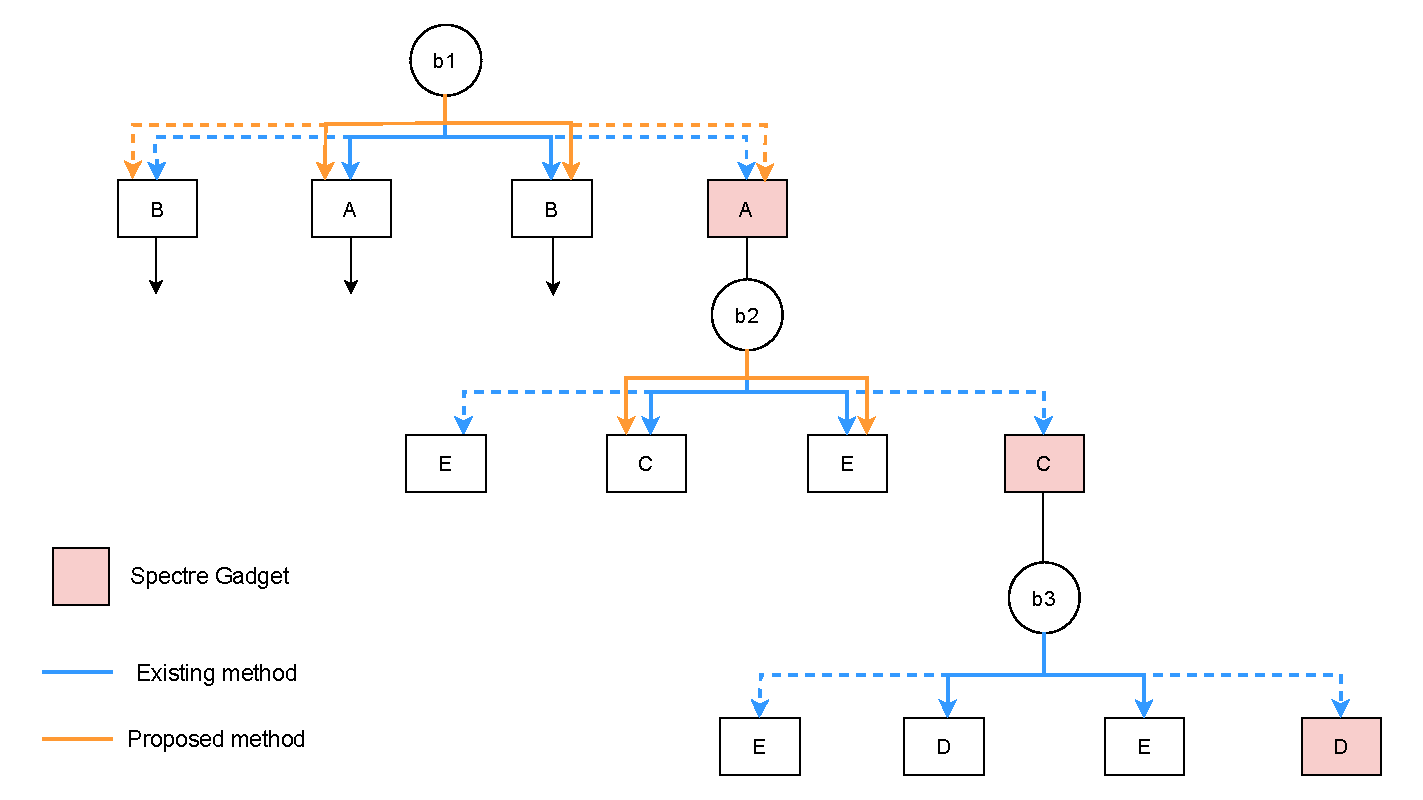
\includegraphics[width=\linewidth]{img/SpecOrder_cfg.drawio.pdf}
  \caption{Order1の記号実行フェーズの解析}\label{fig:SpecOrder_cfg}
\end{figure}

\subsubsection{不要な分岐予測ミスの特定}

記号実行で探索されなかったネストされた分岐予測ミスにより到達する投機的な状態はファジングフェーズで探索を行う。以降は、このような状態をターゲット状態と呼ぶ。この際、ファザーでターゲット状態に到達しない分岐予測ミスをシミュレートすることは非効率的である。\par

図\ref{Unnecessary_branch}に示すコード例を用いて、具体的に説明する。変数\var{index}は攻撃者によって操作可能であり、ファザーによって与えられる入力値を保持すると仮定する。このコード例をファジングフェーズで解析すると、\var{index < ARRAY1\_SIZE}を満たさない入力が\var{index}に与えられた場合、5行目に到達すると分岐予測ミスのシミュレーションが開始し、6行目に実行が進む。その結果、6行目の脆弱性が引き起こされる。しかし、これは1回の分岐予測ミスによって引き起こされる脆弱性であり、Order1の記号実行フェーズですでに検出済みである。その後、シミュレーションは続行されるものの、7行目以降に投機ウィンドウ以上の命令数や直列化命令が存在する場合、8行目に到達する前にシミュレーションが終了し、5行目にロールバックされて正しいパスが実行されることになる。\par

このように、ファジングフェーズにおいて、特定の分岐方向へ分岐予測ミスをシミュレートしても、ターゲット状態に到達できない場合がある。このようなシミュレーションを行っても、記号実行フェーズで既に探索された投機的な状態を再度探索するだけであり、ファジングのスループットを低下させる原因となる。以降ではこのような分岐予測ミスのシミュレーションが不要な分岐方向をRemovable Directionと呼ぶ。記号実行の過程では、このRemovable Directionを特定し、その情報を元にファジングフェーズでは、Removable Directionの分岐予測ミスのシミュレートを抑制する。\par

\begin{figure}
  \begin{minted}[linenos,escapeinside=@@,label=BCB,autogobble]{c}
uint8_t array1[16] = {1, 2, 3, 4, 5, 6, 7, 8, 9, 10, 11, 12, 13, 14, 15, 16}; 
uint8_t array2[256 * 512];
uint8_t temp = 0;
void var(size_t index) {
    if (index < ARRAY1_SIZE) {
       temp &= array2[array1[index] * 512]; // Discovered by symbolic execution
      // lots of code or lfence
      if (condition) {
        // more code
      }
    }
}
   \end{minted}
  \caption{ファジングフェーズにおける分岐予測ミスのシミュレートが不要な例}
  \label{Unnecessary_branch}
\end{figure}

Algorithm\ref{algo_Unnecessary-branch}に記号実行の過程でRemovable Directionを特定するプロセスを示す。各条件分岐命令から分岐予測ミスのシミュレーションが開始された場合、シミュレーションが終了するまでにOrder値(\var{Order})以上の分岐命令に遭遇するかを分岐方向ごとに記録する。記号実行における各状態(\var{$\mu$})は、シミュレーションを開始した分岐命令(\var{missBranch})と分岐予測ミスにより進んだ分岐方向(\var{missDirection})の情報を保持している。また、その分岐方向への分岐予測ミスのシミュレートが不要かどうかを表すフラグ\var{isRemovable}を保持しており、\var{true}に初期化されている。\par

シミュレーション中にOrder値の制限に達した場合、その分岐方向へ分岐予測ミスをシミュレートすることでターゲット状態に到達することを意味するため、\var{isRemovable}を\var{false}にする。最終的に、シミュレーションが終了した際、分岐命令の情報(\var{missBranch, missDirection})と\var{isRemovable} の値を記録する。ただし、同一の分岐命令の分岐方向において、複数の結果が得られた場合(つまり、\var{isRemovable}が\var{true}の場合と\var{false}の場合が存在した場合)、その分岐方向への分岐予測ミスは必要であると保守的に扱う。\par

最終的な結果はJSON形式で図\ref{Unnecessary_branch_result}のように出力される。\var{location}は条件分岐命令の位置を示し、\var{truePath}はその分岐命令のTaken側への分岐予測ミスのシミュレートが不要な場合に\var{true}となる。同様に、\var{falsePath}はNot taken側への分岐予測ミスのシミュレートが必要かを示している。この情報を元に、ファジングフェーズでは分岐予測ミスのシミュレートを抑制する。\par


\begin{figure}
  \begin{algorithm}[H]
    \caption{Removable Directionを特定するアルゴリズム}
    \label{algo_Unnecessary-branch}
\begin{algorithmic}
\State \textbf{Input:}
\State \hspace{1em} $\mu_0$: Initial state
\State \hspace{1em} $\phi_r$: Branch condition for instruction $r$
\State \hspace{1em} SEW: Speculative execution window
\State \hspace{1em} Order: Maximum nested branch misprediction limit

\Function{SYMBOLIC\_EXECUTION}{$\mu_0$, SEW, Order}
\State $\text{states} \gets \{ \mu_0 \}$
\While{$\text{states is not empty}$}
    \State $\mu \gets \text{selectState(states)}$

    \If{$\mu \text{ is speculative state}$ and $\mu.\text{instructionCount} > \text{SEW}$}
        \State $\text{recordMissBranch}(\mu.\text{isRemovable}, \mu.\text{missBranch}, \mu.\text{missDirection})$
        \State $\text{terminateSpState}(\mu)$
        \State \textbf{continue}
    \EndIf

    \State $r \gets \mu.\text{nextInstruction()}$

    \If{$\mu \text{ is speculative state}$}
        \State $\mu.\text{instructionCount} \gets \mu.\text{instructionCount} + 1$
        \If{$r$ is a conditional branch}
            \If{$\mu.\text{missBranchCount} < \text{Order}$}
                \State $\mu_t \gets \text{createSpState}(\mu, \neg\phi_r)$
                \State $\mu_f \gets \text{createSpState}(\mu, \phi_r)$
                \State $\mu_t.\text{missBranchCount} \gets \mu_t.\text{missBranchCount} + 1$
                \State $\mu_f.\text{missBranchCount} \gets \mu_f.\text{missBranchCount} + 1$
                \If{$\mu.\text{missBranchCount} = 1$}
                    \State $\mu_t.\text{missBranch} \gets r$
                    \State $\mu_t.\text{missDirection} \gets \text{true}$
                    \State $\mu_t.\text{isRemovable} \gets \text{false}$
                    \State $\mu_f.\text{missBranch} \gets r$
                    \State $\mu_f.\text{missDirection} \gets \text{false}$
                    \State $\mu_f.\text{isRemovable} \gets \text{false}$
                \EndIf
                \State $\text{states} \gets \text{states} \cup \{ \mu_t, \mu_f \}$
            \Else
                \State $\mu.\text{isRemovable} \gets \text{false}$
            \EndIf
        \EndIf

        \If{$r$ is Exit or Fence}
            \State $\text{recordMissBranch}(\mu.\text{isRemovable}, \mu.\text{missBranch}, \mu.\text{missDirection})$
            \State $\text{terminateSpState}(\mu)$
        \EndIf
    \EndIf
\EndWhile
\EndFunction
\end{algorithmic}
\end{algorithm}

\end{figure}

\begin{figure}
  \begin{lstlisting}[language=json]
{
  "branches": [
    {
      "location": "/path/sample.c:12",
      "truePath": false,
      "falsePath": true,
    },
    {
      "location": "/path/sample.c:18",
      "truePath": true,
      "falsePath": false,
    }
    ...
  ]
}
  \end{lstlisting}
  \caption{Removable Directionを特定した結果}
  \label{Unnecessary_branch_result}
\end{figure}


\subsubsection{ターゲット状態までの実行トレースの取得}
ファジングフェーズでは、ターゲット状態に到達する入力を効率的に生成することが求められる。そのため、テストケースがターゲット状態に到達する可能性を評価するための指標が必要となる。その指標として、記号実行フェーズにおいて、ターゲット状態に至るまでに通過した分岐方向(分岐予測ミスも含む)の実行トレースを収集する。以降ではこのような分岐方向をTarget Directionと呼ぶ。この情報を基に、ファジングフェーズではテストケースがTarget Directionをどれだけ通過できたかで、そのテストケースの有効性を評価する。\par

記号実行では、各状態は、通過した分岐命令と進んだ分岐方向の情報を保持している。Orderの制限に達した時点で、その状態が保持する分岐情報のトレースをグローバルなデータ構造に記録する。最終的に、各分岐命令の分岐方向ごとに、ターゲット状態に到達するまでにその分岐方向を一度でも通過したかどうかを集計し、Target DirectionをJSON形式でファイルに出力する。\par

図\ref{Execution_Trace}に出力されるJSONファイルの内容を示す。\var{location}は条件分岐命令の位置を示し、その後分岐予測ミスを含んだ各分岐方向(\var{truePath,falsePath,trueSpPath,falseSpPath})に対し、ターゲット状態に到達するまでにその分岐方向を一度でも通過した場合は1を、通過しなかった場合は0が記録される。\var{Sum}はターゲット状態に到達するまでに通過した分岐方向(すなわち1が記録されている分岐方向)の総数を表す。この情報を元に、ファジングフェーズではテストケースの有効性を評価する。\par

\begin{figure}
  \begin{lstlisting}[language=json]
{
    "branches": [
        {
            "location": "/path/sample.c:9",
            "truePath": 1,
            "falsePath": 0,
            "trueSpPath": 0,
            "falseSpPath": 0
        },
        {
            "location": "/path/sample.c:21",
            "truePath": 1,
            "falsePath": 1,
            "trueSpPath": 0,
            "falseSpPath": 1
        },
       ...
    ],
    "Sum": 14
}
  \end{lstlisting}
  \caption{Target Directionを取得した結果}
  \label{Execution_Trace}
\end{figure}

\subsection{ファジングフェーズ}

\subsubsection{不要な分岐予測ミスの抑制}
ファジングフェーズでは、記号実行で探索されなかったターゲット状態を集中的に探索したい。その際、ターゲット状態に到達しない分岐予測ミスをシミュレートすることは非効率的である。そこで、記号実行フェーズで得られた結果\ref{Unnecessary_branch_result}を用い、Removable Directionの分岐予測ミスのシミュレートを抑制する。\par
提案手法はLLVMのMIRレベルでの計装によって行われる。図\ref{fig:Fuzzing_Phase_cfg}に計装前の制御フローグラフと、分岐予測ミスを抑制した計装後の制御フローグラフの概略図を示す。分岐予測ミスのシミュレート用の計装はSpecFuzzと同様である。詳しくは\ref{sec:specfuzz}を参照されたい。提案手法では、記号実行フェーズの結果から、Removable Directionであると判断された分岐方向に対応する基本ブロックの先頭に、\var{force\_rlbk()}という関数の呼び出しを挿入する。
この関数は、直前の分岐命令においてシミュレーションが開始されていた場合に、シミュレートを終了し、強制的にロールバックさせる関数である。このような計装を行うことで、投機ウィンドウの上限に達するのを待たずにシミュレーションを終了できるため、記号実行で既に探索済みの投機的な状態を再度探索することをできるだけ回避する。その結果、ファジングフェーズのスループット向上が期待される。\par

\begin{figure}[tb]
  \centering
  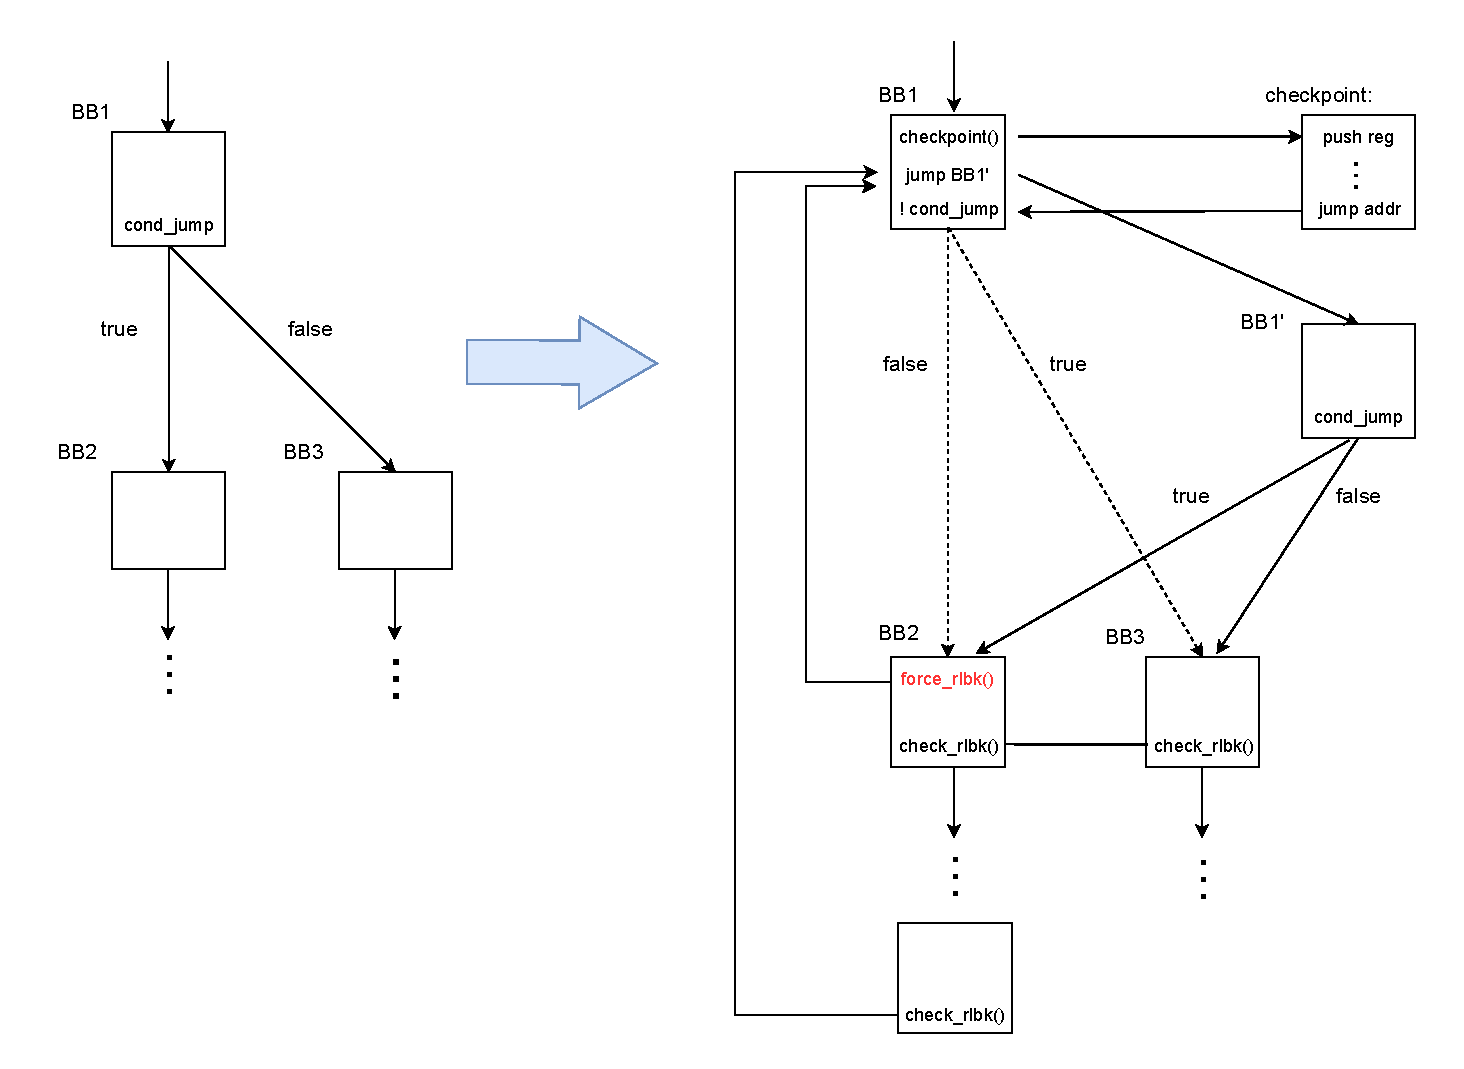
\includegraphics[width=\linewidth]{img/Fuzzing_Phase.drawio.pdf}
  \caption{計装によるRemovable Directionの分岐予測ミスの抑制}\label{fig:Fuzzing_Phase_cfg}
\end{figure}

\subsubsection{スコアによるシードのスケジューリング}
ファジングフェーズでは、ターゲット状態に到達する入力を効率的に生成することが求められる。そこで、記号実行フェーズで得られた結果\ref{Execution_Trace}を用いて、テストケースがTarget Directionをどれだけ通過したかでテストケースの有効性を評価する。ファジングフェーズでは、LLVMのMIRレベルでの計装によって、テストケースが通過した分岐命令と分岐方向(分岐予測ミスも含む)を記録するようにする。そして、式\ref{equ:Scoring}により導出した値の小数点以下を四捨五入した値をテストケースのスコアとする。

\begin{equation}
\text{スコア} = \left( \frac{\text{テストケースが通過したTarget Directionの種類数}}
{\text{Target Directionの総数}} \right) \times 10
  \label{equ:Scoring}
\end{equation}
\vspace{1em}

通過した分岐方向の種類数をスコア計算に使用するため、ループなどの影響で同一の分岐方向に複数回通過しても、一度しかカウントしない。これにより、テストケースがループなどによって不適切に高いスコアを獲得することを防ぐ。このスコアをファザーへのフィードバックとして提供する。ファザーは高いカバレッジを獲得したテストケースに加え、より高いスコアを獲得したテストケースもシードコーパスに追加する。また、シードが保持するスコアが高いほど、そのシードを元に変異によって生成される新しいテストケース数を増やすようにする。図\ref{fig:seed_schedule}にスコアを用いたシードのスケジューリング戦略の概要を示す。こうすることで、ファザーはターゲット状態に到達する可能性の高いテストケースを優先的に実行できると考える。

\begin{figure}[tb]
  \centering
  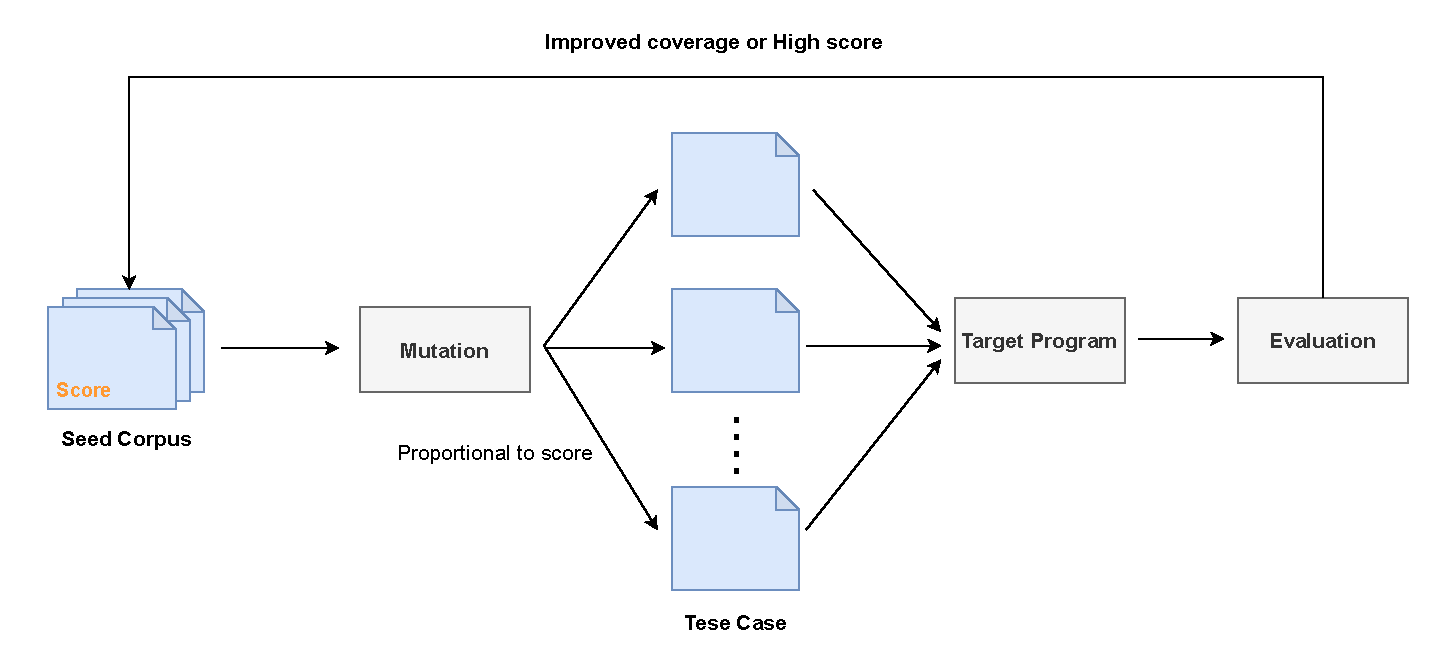
\includegraphics[width=\linewidth]{img/seed_schedule.drawio.pdf}
  \caption{スコアを用いたシードのスケジューリング戦略}\label{fig:seed_schedule}
\end{figure}






